\documentclass[a4paper, 12pt]{article}
\usepackage[top=2cm, bottom=2cm,left=2.5cm, right=2.5cm]{geometry}
\usepackage[utf8]{inputenc}
\usepackage{amsmath, amsfonts, amssymb}
\usepackage{float}
\usepackage{graphicx}
\renewcommand*\contentsname{Sum\'ario}
\begin{document}

\title{Trabalho 02 - Programa\c{c}\~ao em linguagem do Montagem MIPS: Aritm\'etica de inteiros}
\author{Adailson Pinho dos Santos - 13/0140724\\
Vitor Nere Ara\'ujo Ribeiro - 13/0137413}
\date{}
\maketitle

\newpage

\tableofcontents

\newpage

\section{Introdu\c{c}\~ao}
	\paragraph{}	Este documento tem como objetivo relatar o desenvolvimento do trabalho 2 da mat\'eria Fundamentos de Arquitetura de Software, descreve tamb\'em qual ambiente de desenvolvimento utilizado e quais s\~ao as instru\c{c}\~oes de uso. 
	\paragraph{}	O trabalho 2 consiste em desenvolver um programa em linguagem de montagem Assembly MIPS que realize o c\'alculo do inverso multiplicativo a partir da leitura de dois n\'umeros, o primeiro sendo o prov\'avel n\'umero primo (m\'odulo) e o segundo sendo um n\'umero inteiro, ao final, o sistema deve imprimir uma mensagem do resultado do inverso multiplicativo ou uma mensagem que informa que o m\'odulo n\~ao \'e primo. 
\section{Ambiente de desenvolvimento}
    \paragraph{}	Para a execu\c{c}\~ao do desenvolvimento das aplica\c{c}\~oes foram utilizados os Sistemas Operacionais Fedora 26 e Debian 9, sendo que ambos s\~ao distribui\c{c}\~oes populares do Linux. 
    \paragraph{}	Foi utilizado o simulador de MARS para programar em linguagem de montagem MIPS, a vers\~ao utilizada foi a v4.5 disponibilizada em agosto de 2014, esse software que foi desenvolvido em Java foi essencial para o desenvolvimendo do trabalho. A vers\~ao do Java(TM) SE Runtime Environment utilizado para a execu\c{c}\~ao do simulador MARS foi a v1.8.0.
\section{Constru\c{c}\~ao}
\paragraph{}	A n\'ivel de constru\c{c}\~ao do software a dupla utilizou os procedimentos: \_\_start, ler\_inteiro, eh\_primo, calc\_inverso, imprime\_erro e imprime\_saida. No c\'odigo fonte s\~ao descritos os coment\'arios relativos ao funcionamento de cada procedimento e suas rela\c{c}\~oes.
\paragraph{}	A equipe utilizou apenas as seguintes instru\c{c}\~oes: jal, slti, beq, bne, li, la, syscall, move, jr, addi, div, mfhi, j, mult, mflo.

\section{Racioc\'inio l\'ogico} 
    \paragraph{}	Em matem\'atica modular o n\'umero \'e considerado inverso multiplicativo quando: \begin{equation} A(mod C) = A^{-1} \end{equation} ou  \begin{equation} (A * A^-1) \equiv 1 \pmod{c} \end{equation} 
    \paragraph{}	Dessa forma, \'e necess\'ario percorrer o valor do resto da divis\~ao pelo m\'odulo em cada n\'umero multiplicativo at\'e que o resto seja 1, quando isso acontecer o inverso modular \'e o n\'umero multiplicativo.
        
\section{Instru\c{c}\~ao de uso}
		\paragraph{}    Primeiramente, se deve baixar o MARS Simulator no site do MARS e entrar na pasta onde se encontra o MARS: 
		\begin{figure}[H]
			\centering
			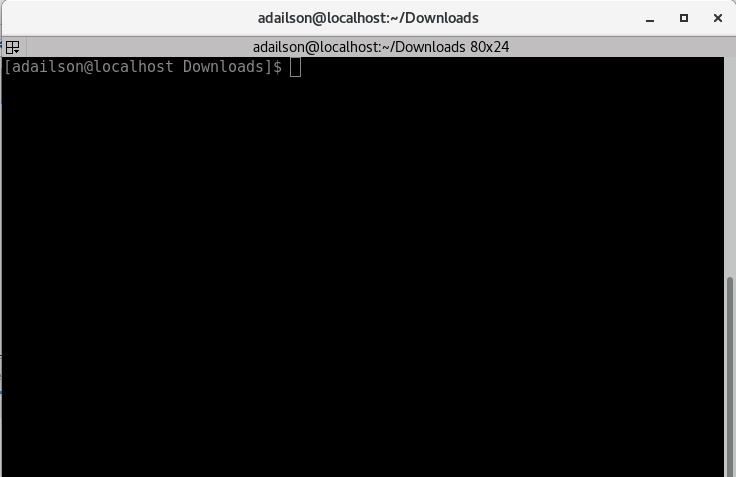
\includegraphics[scale=0.5]{img1.png}
		\end{figure}
		\paragraph{}    Executar o simulador da seguinte forma:
		\begin{figure}[H]
			\centering
			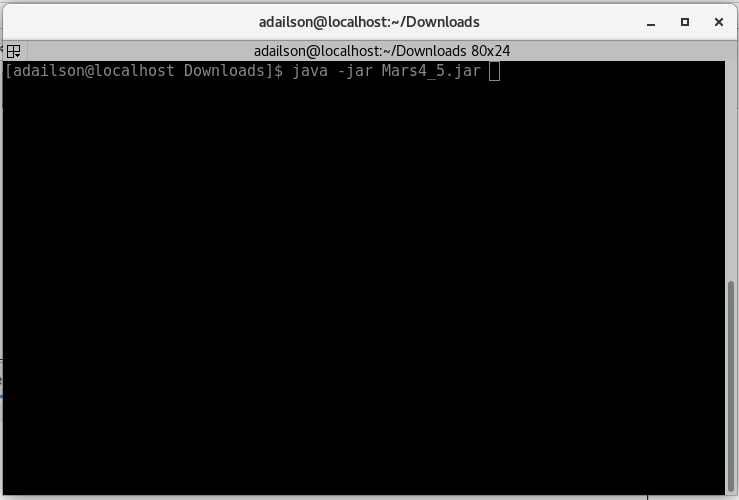
\includegraphics[scale=0.5]{img2.png}
		\end{figure}
        \paragraph{}    Com o MARS simulator aberto, o usu\'ario deve abrir o arquivo .ASM que cont\'em as instru\c{c}\~oes em Assembly MIPS:
        \begin{figure}[H]
        	\centering
        	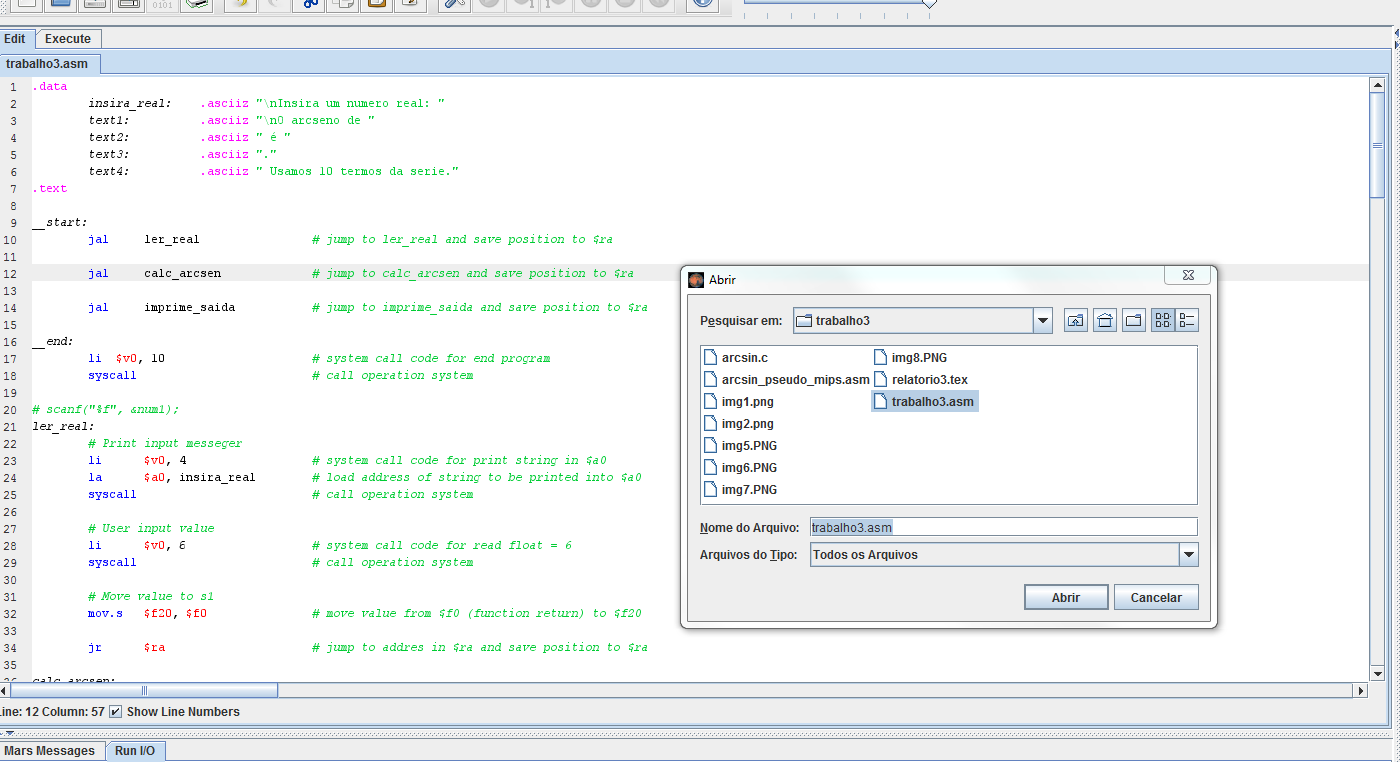
\includegraphics[scale=0.3]{img3.png}
        \end{figure}
        \paragraph{}    Agora, o usu\'ario deve clicar na Aba Run-Assemble para montar o programa e Run-Go para executar o programa. Para a primeira tela, \'e dado para o primeiro inteiro e prov\'avel primo o n\'umero 5 e para o segundo inteiro o n\'umero 2, a resposta deve consistir em: "O inverso multiplicativo \'e 3.":
        \begin{figure}[H]
        	\centering
        	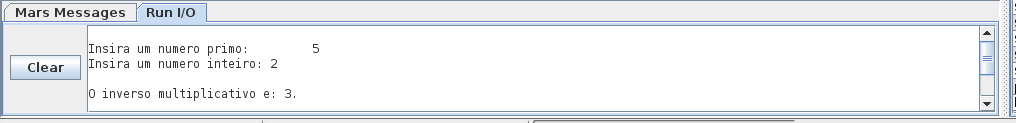
\includegraphics[scale=0.5]{img4.png}
        \end{figure}
        \paragraph{}    Na segunda tela, \'e dado para o primeiro inteiro e prov\'avel primo o n\'umero 12 e para o segundo inteiro o n\'umero 3, A resposta deve consistir: "O modulo nao eh primo.":
        \begin{figure}[H]
        	\centering
        	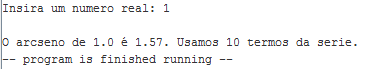
\includegraphics[scale=0.5]{img5.png}
        \end{figure}
        \paragraph{}    
\end{document}